\documentclass[tikz,border=8pt]{standalone}
% Shared preamble for the bootqcc TikZ figures.
\usepackage[T1]{fontenc}
\usepackage{helvet}
\renewcommand{\familydefault}{\sfdefault}
\usepackage{amsmath}
\usetikzlibrary{arrows.meta,positioning,shapes.geometric,fit,backgrounds,calc}

\definecolor{navy}{HTML}{1F3A5F}
\definecolor{sky}{HTML}{5AA9E6}
\definecolor{coral}{HTML}{FF6B6B}
\definecolor{slate}{HTML}{6B7A8F}

\tikzset{
  box/.style={rectangle, rounded corners=4pt, draw=navy, fill=sky!15, thick,
              align=center, minimum height=1.0cm, inner sep=6pt, text width=4.6cm},
  inbox/.style={rectangle, rounded corners=4pt, draw=slate, fill=slate!10, thick,
              align=center, minimum height=0.9cm, inner sep=5pt, text width=3.0cm,
              font=\small},
  io/.style={trapezium, trapezium left angle=72, trapezium right angle=108,
             draw=navy, fill=white, thick, align=center, minimum height=1.2cm,
             inner sep=5pt, text width=3.0cm},
  result/.style={rectangle, rounded corners=8pt, draw=coral, fill=coral!10, thick,
              align=center, minimum height=1.0cm, inner sep=6pt, text width=4.0cm},
  term/.style={rectangle, rounded corners=12pt, draw=navy, fill=navy, text=white,
               thick, align=center, minimum height=0.9cm, inner sep=6pt, text width=4.2cm},
  dec/.style={diamond, aspect=2.6, draw=navy, fill=white, thick, align=center,
              inner sep=0pt, text width=2.7cm, font=\small},
  err/.style={rectangle, rounded corners=4pt, draw=coral, fill=coral!15, thick,
              align=center, minimum height=0.9cm, inner sep=6pt, text width=3.2cm},
  arr/.style={-{Latex[length=3mm]}, thick, navy},
  lab/.style={font=\footnotesize\bfseries, text=navy, fill=white, inner sep=1.5pt},
  phase/.style={rounded corners=8pt, draw=navy!45, dashed, thick, inner sep=12pt},
}

\begin{document}
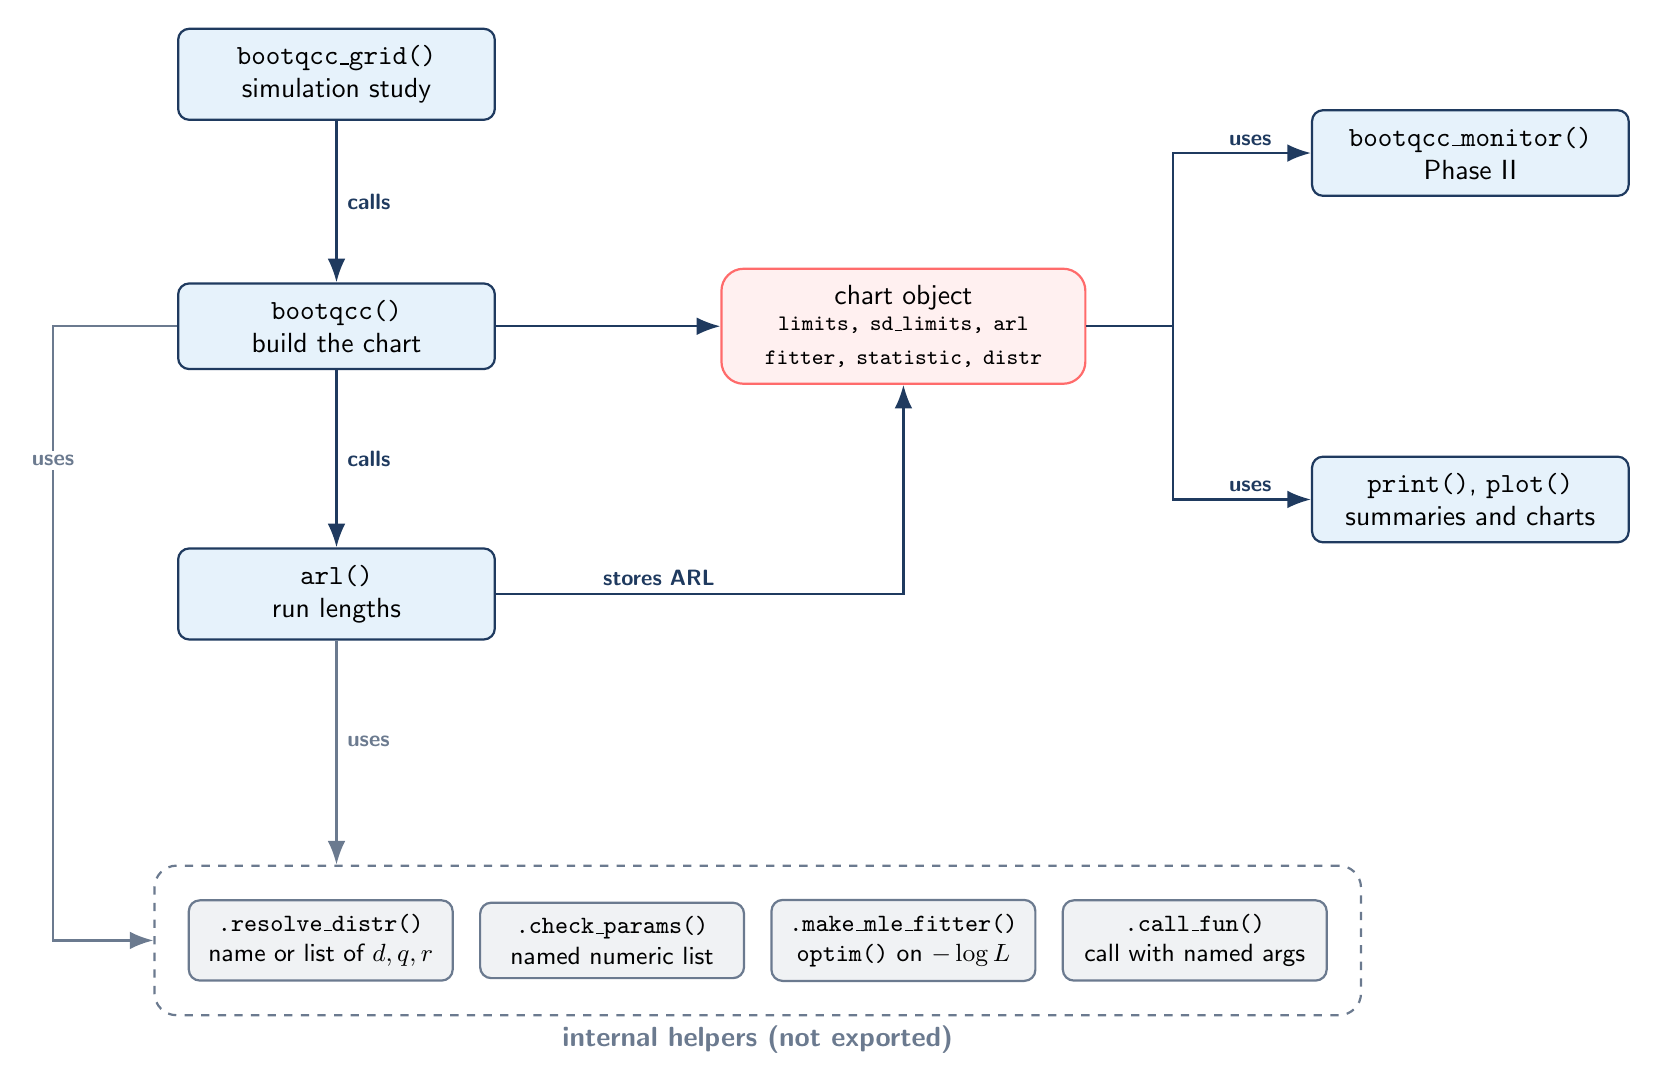
\begin{tikzpicture}

  % user-facing functions
  \node[box, text width=3.6cm] (grid) at (0,6.4)  {\texttt{bootqcc\_grid()}\\ simulation study};
  \node[box, text width=3.6cm] (main) at (0,3.2)  {\texttt{bootqcc()}\\ build the chart};
  \node[box, text width=3.6cm] (arl)  at (0,-0.2) {\texttt{arl()}\\ run lengths};
  \node[result, text width=4.2cm] (obj) at (7.2,3.2)
    {chart object\\ \footnotesize \texttt{limits, sd\_limits, arl}\\ \texttt{fitter, statistic, distr}};
  \node[box, text width=3.6cm] (mon) at (14.4,5.4) {\texttt{bootqcc\_monitor()}\\ Phase II};
  \node[box, text width=3.6cm] (pp)  at (14.4,1.0) {\texttt{print()}, \texttt{plot()}\\ summaries and charts};

  % internal helpers
  \node[inbox] (h1) at (-0.2,-4.6) {\texttt{.resolve\_distr()}\\ name or list of $d,q,r$};
  \node[inbox] (h2) at (3.5,-4.6)  {\texttt{.check\_params()}\\ named numeric list};
  \node[inbox] (h3) at (7.2,-4.6)  {\texttt{.make\_mle\_fitter()}\\ \texttt{optim()} on $-\log L$};
  \node[inbox] (h4) at (10.9,-4.6) {\texttt{.call\_fun()}\\ call with named args};

  \begin{pgfonlayer}{background}
    \node[phase, draw=slate, fit=(h1)(h2)(h3)(h4), name=helpers,
          label={[slate,font=\bfseries]below:internal helpers (not exported)}] {};
  \end{pgfonlayer}

  % calls between the user-facing functions
  \draw[arr] (grid) -- node[lab, right=2pt, pos=0.5] {calls} (main);
  \draw[arr] (main) -- node[lab, right=2pt, pos=0.5] {calls} (arl);
  \draw[arr] (main) -- (obj);
  \draw[arr] (arl.east) -| node[lab, pos=0.2, above=1pt] {stores ARL} (obj.south);

  % the chart object feeds Phase II and the print/plot methods
  \draw[arr] (obj.east) -- ++(1.1,0) |- node[lab, pos=0.78, above=1pt] {uses} (mon.west);
  \draw[arr] (obj.east) -- ++(1.1,0) |- node[lab, pos=0.78, above=1pt] {uses} (pp.west);

  % helpers
  \draw[arr, slate] (main.west) -- (-3.6,3.2) |- node[lab, pos=0.12, above=1pt, text=slate] {uses} (helpers.west);
  \draw[arr, slate] (arl.south) -- node[lab, right=2pt, pos=0.45, text=slate] {uses} (arl.south |- helpers.north);
\end{tikzpicture}
\end{document}
